\documentclass[polish,polish,a4paper]{article}
\usepackage[utf8]{inputenc}
\usepackage[T1]{fontenc}
\usepackage{polski}
\usepackage{anysize}
\usepackage{siunitx}
\usepackage{graphicx}
\usepackage{xcolor} % do komentarzy

\marginsize{2.5cm}{2.5cm}{3cm}{3cm}

\title{Symulator tomografu komputerowego}
\author{Przemysław Ambroży, Błażej Celmer}

\begin{document} 
	\maketitle
	
 	\section{Model}
		\begin{center}
			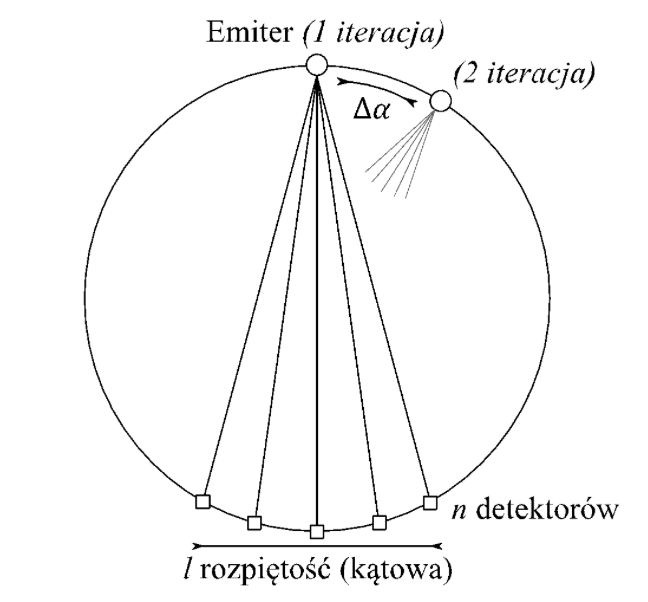
\includegraphics[scale=0.7]{img/model.png} \\
			\small{rys. 1. model stożkowy}
		\end{center}
		Zastosowany został model stożkowy (rys. 1.).
		 Zakłada on wykorzystanie jednego emitera,
		  który współpracuje ze wszystkimi detektorami, tworząc wspomniany stożek 
		  (W przeciwieństwie do modelu równoległego, gdzie każdy detektor posiada własny emiter).
		 {\color{red}  coś bym tu jeszcze dopisał }
		
	\section{Program}
		\subsection{Środowisko}
			Do zasymulowania tomografu skorzystaliśmy z języka Python w środowisku Jupyter Notebook,
			 co pozwoliło niskim kosztem uzyskać interfejs użytkownika.
			 Skorzystaliśmy również z bibliotek, które oferowały dodatkowe funkcjonalności:
			
			\begin{description}
				\item[matplotlib] wyświetlanie grafik
				\item[ipywidgets] interfejs użytkownika
				\item[pydicom] odczyt i zapis plików DICOM
			\end{description}
			{\color{red} w sumie to nie wiem czy trzeba wszystkie wypisywać (chyba, że coś ważnego w tych bibliotekach)}
	
			\subsection{Opis działania}
				\subsubsection{Sinogram}
				
				Sinogram, jest to tablica danych, 
				gdzie każdy wiersz to jedna iteracja, 
				a każda kolumna oznacza jeden detektor.
				Aby go otrzymać, należy wykonać n iteracji, 
				w których emiter w raz z detektorami będzie się stopniowo przesuwał po okręgu, 
				aż obrócimy cały system o 180 stopni. 
				Podczas każdej iteracji, 
				pobieramy dane z obiektu znajdującego się między emiterem, a detektorami
				 - w naszym przypadku jest to obraz. 
				 {\color{red} Opis algorytmu wyznaczania linii.}
				 Znając wszystkie piksele leżące między emiterem, a detektorem, 
				 sumujemy ich jasność i zapisujemy w odpowiednim miejscu w sinogramie.
				 Na koniec należy znormalizować wszystkie dane, tak aby wartości były z przedziału od 0 do 1.
				{\color{red} gdzieś trzeba wkleić kawałki kodu, pewnie trzeba będzie to podzielić i dopisać więcej}
				
				\subsubsection{Obraz wynikowy}
				Sinogram nie jest zrozumiały dla człowieka, 
				dlatego należy go przekształcić.
				Zaczynamy od czarnego obrazu i znów przejdziemy przez n iteracji.
				Każdej iteracji przypisana będzie pozycja emitera wraz z detektorami 
				(będą to te same pozycje, co podczas generowania sinogramu).
				Wyznaczamy linie przechodzące przez obraz między emiterem i detektorami (algorytm Bresenhama).
				Każdy piksel, przez który przechodzi linia będzie rozjaśniony o wartość odczytaną z sinogramu 
				(dla danego detektora w danej iteracji). 
				Nałożenie wszystkich linii na obrazie stworzy obraz wynikowy.
				{\color{red} to samo co wyżej, no i myślę jeszcze o jakiś obrazkach}
			\subsection{Standard DICOM}
\end{document}
